%* glpk-java.tex *%

%***********************************************************************
%  This code is part of GLPK for Java.
%
%  Copyright (C) 2009, 2010, 2011 Heinrich Schuchardt,
%  <xypron.glpk@gmx.de>
%
%  GLPK for Java is free software: you can redistribute it and/or 
%  modify it under the terms of the GNU General Public License as
%  published by the Free Software Foundation, either version 3 of the
%  License, or (at your option) any later version.
%
%  GLPK for Java is distributed in the hope that it will be useful, but 
%  WITHOUT ANY WARRANTY; without even the implied warranty of 
%  MERCHANTABILITY or FITNESS FOR A PARTICULAR PURPOSE. See the GNU 
%  General Public License for more details.
%
%  You should have received a copy of the GNU General Public License
%  along with GLPK for Java. If not, see <http://www.gnu.org/licenses/>.
%***********************************************************************

%\documentclass[dvipdfm,11pt]{report}
%\usepackage[dvipdfm,linktocpage,colorlinks,linkcolor=blue,urlcolor=blue]{hyperref}
\documentclass[a4paper,11pt]{report}
\usepackage{hyperref}
\usepackage{parskip}
\usepackage{natbib}
\usepackage{url}
\usepackage{graphicx}
\usepackage{pdflscape}
\usepackage[top=2cm, bottom=2cm, left=2cm, right=2cm]{geometry}
\usepackage{makeidx}
%%generate index
\makeindex

\renewcommand\contentsname{\sf\bfseries Contents}
\renewcommand\chaptername{\sf\bfseries Chapter}
\renewcommand\appendixname{\sf\bfseries Appendix}

\setlength{\parindent}{0pt}
\setlength{\parskip}{10pt} 

\begin{document}

\thispagestyle{empty}

\begin{center}

\vspace*{1in}

\begin{huge}
\sf\bfseries GNU Linear Programming Kit\linebreak
Java Binding
\end{huge}

\vspace{0.5in}

\begin{LARGE}
\sf Reference Manual
\end{LARGE}

\vspace{0.5in}

\begin{LARGE}
\sf Version 1.0.18
\end{LARGE}

\vspace{0.5in}
\begin{Large}
\sf September 2011
\end{Large}
\end{center}

\newpage

\vspace*{1in}

\vfill

\medskip \noindent
Copyright \copyright{} 2009, 2010, 2011 Heinrich Schuchardt,
xypron.glpk@gmx.de

\medskip \noindent
Permission is granted to make and distribute verbatim copies of this
manual provided the copyright notice and this permission notice are
preserved on all copies.

\medskip \noindent
Permission is granted to copy and distribute modified versions of this
manual under the conditions for verbatim copying, provided also that the
entire resulting derived work is distributed under the terms of
a permission notice identical to this one.

\medskip \noindent
Permission is granted to copy and distribute translations of this manual
into another language, under the above conditions for modified versions.

\medskip \noindent
Windows is a registered trademark of Microsoft Corporation. Java is a 
trademark when it identifies a software product of Sun Microsystems, Inc.

\tableofcontents

\chapter{Introduction}
The GNU Linear Programming Kit (GLPK)\cite{GLPK} package supplies a solver for
large scale linear programming (LP) and mixed integer programming (MIP). The
GLPK project is hosted at
\linebreak\href{http://www.gnu.org/software/glpk}{http://www.gnu.org/software/glpk}.

It has two mailing lists:\index{support}
\begin{itemize}
\item\href{mailto:help-glpk@gnu.org}{help-glpk@gnu.org} and 
\item\href{mailto:bug-glpk@gnu.org}{bug-glpk@gnu.org}.
\end{itemize}
To subscribe to one of these lists, please, send an empty mail with a Subject: header line of just "subscribe" to the list.

GLPK provides a library written in C and a standalone solver.

The source code provided at \href{ftp://gnu.ftp.org/gnu/glpk/}{ftp://gnu.ftp.org/gnu/glpk/} contains the documentation of the library in  file doc/glpk.pdf.

The Java platform provides the Java Native Interface (JNI)\cite{JNI} to integrate non-Java language libraries into Java applications.

Project GLPK for Java delivers a Java Binding for GLPK. It is hosted at \linebreak\href{http://glpk-java.sourceforge.net/}{http://glpk-java.sourceforge.net/}.

To report problems and suggestions concerning GLPK for Java, please, send an email to the author at \href{mailto:xypron.glpk@gmx.de}{xypron.glpk@gmx.de}\index{support}.

\chapter{Architecture}
A GLPK for Java application will consist of the following
\begin{itemize}
\item the GLPK library
\item the GLPK for Java JNI library
\item the GLPK for Java class library
\item the application code.
\end{itemize}

\section{GLPK library}

\subsection{Source}
The source code to compile the GLPK library is provided at \linebreak\href{ftp://gnu.ftp.org/gnu/glpk/}{ftp://gnu.ftp.org/gnu/glpk/}.

\subsection{Linux}
\index{Linux}
The GLPK library can be compiled from source code. Follow the instructions in file INSTALL provided in the source distribution. Precompiled packages are available in many Linux distributions.

The usual installation path for the library is /usr/local/lib/libglpk.so.
\subsection{Windows}
\index{Windows}
The GLPK library can be compiled from source code. The build and make files are in directory w32 for 32 bit Windows and in w64 for 64 bit Windows. The name of the created library is glpk\_4\_47.dll for revision 4.47.

A precompiled version of GLPK is provided at \href{http://winglpk.sourceforge.net}{http://winglpk.sourceforge.net}.

The library has to be in the search path for binaries. Either copy the library to a directory that is already in the path (e.g. C:\textbackslash windows\textbackslash system32) or update the path in the system settings of Windows.

\section{GLPK for Java JNI library}
\index{JNI library}
\subsection{Source}
The source code to compile the GLPK for Java JNI library is provided at \linebreak\href{http://glpk-java.sourceforge.net}{http://glpk-java.sourceforge.net}.

\subsection{Linux}
\index{Linux}
The GLPK for Java JNI library can be compiled from source code. Follow the instructions in file INSTALL provided in the source distribution.

The usual installation path for the library is /usr/local/lib/libglpk-java.so.
\subsection{Windows}
\index{Windows}
The GLPK for Java JNI library can be compiled from source code. The build and make files are in directory w32 for 32 bit Windows and in w64 for 64 bit Windows. The name of the created library is glpk\_4\_47\_java.dll for revision 4.47.

A precompiled version of GLPK for Java is provided at \linebreak\href{http://winglpk.sourceforge.net}{http://winglpk.sourceforge.net}.

The library has to be in the search path for binaries. Either copy the library to a directory that is already in the path (e.g. C:\textbackslash windows\textbackslash system32) or update the path in the system settings of Windows.

\section{GLPK for Java class library}
The source code to compile the GLPK for Java class library is provided at \linebreak\href{http://glpk-java.sourceforge.net}{http://glpk-java.sourceforge.net}.

\subsection{Linux}
\index{Linux}
The GLPK for Java class library can be compiled from source code. Follow the instructions in file INSTALL provided in the source distribution.

The usual installation path for the library is /usr/local/share/java/glpk-java.jar.

For Debian and Ubuntu the following packages are needed for compilation:
\begin{itemize}
	\item libtool
	\item swig
	\item java-gcj-compat-dev
\end{itemize}
\subsection{Windows}
\index{Windows}
The GLPK for Java class library can be compiled from source code. The build and make files are in directory w32 for 32 bit Windows and in w64 for 64 bit Windows. The name of the created library is glpk-java.jar.

A precompiled version of GLPK including GLPK-Java is provided at \linebreak\href{http://winglpk.sourceforge.net}{http://winglpk.sourceforge.net}.

\subsection{Classpath}
\index{classpath}
The library has to be in the CLASSPATH. Update the classpath in the system settings of Windows or specify the classpath upon invocation of the application, e.g.
\begin{verbatim}
java -classpath ./glpk-java.jar;. MyApplication
\end{verbatim}
\chapter{Classes}
\index{classes}
GLPK for Java uses the Simplified Wrapper and Interface Generator (SWIG)\index{SWIG}\cite{SWIG} to create
the JNI interface to GLPK.
\index{class path}
Classes are created in path org.gnu.glpk.

Class GlpkCallback is called by the MIP solver callback routine.

Interface GlpkCallbackListener can be implemented to register a listener for
class GlpkCallback.

Class GlpkTerminal is called by the MIP solver terminal output routine.

Interface GlpkTerminalListener can be implemented to register a listener for
class GlpkTerminal.

Class GlpkException is thrown if an error occurs.

Class GLPK maps the functions from glpk.h.

Class GLPKConstants maps the constants from glpk.h to methods.

Class GLPKJNI contains the definitions of the native functions.

The following classes map structures from glpk.h:
\begin{itemize}
\item glp\_attr
\item glp\_bfcp
\item glp\_cpxcp
\item glp\_data
\item glp\_iocp
\item glp\_iptcp
\item glp\_long
\item glp\_mpscp
\item glp\_prob
\item glp\_smcp
\item glp\_tran
\item glp\_tree
\item LPXKKT
\item \_glp\_arc
\item \_glp\_graph
\item \_glp\_vertex
\end{itemize}

The following classes are used to map pointers:
\begin{itemize}
\item SWIGTYPE\_p\_double
\item SWIGTYPE\_p\_f\_p\_glp\_tree\_p\_void\_\_void
\item SWIGTYPE\_p\_f\_p\_q\_const\_\_char\_v\_\_\_\_\_\_\_void
\item SWIGTYPE\_p\_f\_p\_void\_\_void
\item SWIGTYPE\_p\_f\_p\_void\_p\_q\_const\_\_char\_\_int
\item SWIGTYPE\_p\_int
\item SWIGTYPE\_p\_p\_\_glp\_vertex
\item SWIGTYPE\_p\_va\_list
\item SWIGTYPE\_p\_void
\end{itemize}

\chapter{Usage}
Please, refer to file doc/glpk.pdf of the GLPK source distribution for a detailed description of the methods and constants.

\section{Loading the JNI library}
\index{JNI library}
To be able to use the JNI library in a Java program it has to be loaded.
The path to dynamic link libaries can specified on the command line when
calling the Java runtime, e.g.
\begin{verbatim}
java -Djava.library.path=/usr/local/lib/jni/libglpk_java
\end{verbatim}

The following code is used in class GLPK to load the JNI library:

\begin{verbatim}
static {
  try {
    if (System.getProperty("os.name").toLowerCase().contains("windows")) {
      // try to load Windows library
      System.loadLibrary("glpk_4_47_java");
    } else {
      // try to load Linux library
      System.loadLibrary("glpk_java");
    }
  } catch (UnsatisfiedLinkError e) {
    System.err.println(
      "The dynamic link library for GLPK for Java could not be"
      + "loaded.\nConsider using\njava -Djava.library.path=");
    throw e;
  }
}
\end{verbatim}

If the JNI library can not be loaded, you will receive an exception
\linebreak java.lang.UnsatisfiedLinkError.

\section{Exceptions}
\index{exceptions}
\index{GlpkException}
When illegal parameters are passed to a function of the GLPK native library
an exception GlpkException is thrown. Due to the architecture of GLPK all
GLPK objects are invalid when such an exception has occured.

\subsection{Implementation details}
GLPK for Java registers a function glp\_java\_error\_hook() to glp\_error\_hook()
before calling an GLPK API function. If an error occurs function glp\_free\_env
is called and a long jump is used to return to the calling environment. Then
function glp\_java\_throw() is called which throws GlpkException.

\section{Callbacks}
\index{callbacks}
\index{GlpkCallback}
\index{GlpkCallbackListener}
The MIP solver provides a callback functionality. This is used to call
method callback of class GlpkCallback. A Java program can listen to the
callbacks by instantiating a class implementing interface
GlpkCallbackListener and registering the object with method addListener()
of class GlpkCallback. The listener can be deregistered with method
removeListener(). The listener can use method GLPK.glp\_ios\_reason() to find
out why it is called. For details see the GLPK library documentation.

\begin{landscape}
\begin{figure}[swimlanes]
\caption{Callbacks and Error Handling}
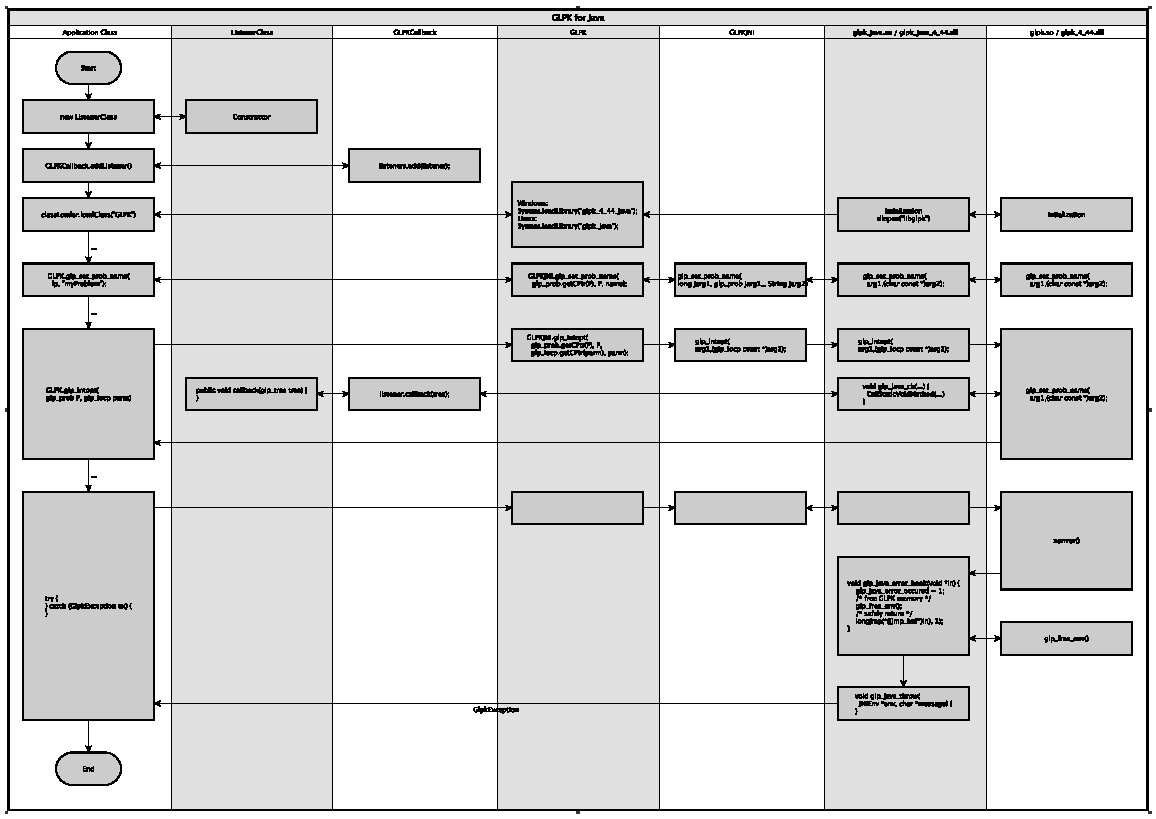
\includegraphics[scale=1.2]{swimlanes.pdf}
\end{figure}
\end{landscape}

\section{Output listener}
\index{output listener}
\index{GlpkTerminal}
\index{GlpkTerminalListener}
GLPK provides a hook for terminal output. A Java program can listen to the
callbacks by instantiating a class implementing interface GlpkTerminalListener
and registering the object with method addListener of class GlpkTerminal.
The listener can be dregistered with method removeListener().
After a call to glp\_free\_env() the GlpkTerminal has to registered again
by calling GLPK.glp\_term\_hook(null, null). glp\_free\_env() is called if
an exception GlpkException occurs.

\section{Aborting a GLPK library call}
\index{abort}
\index{GlpkException}
\index{glp\_java\_error}
Method void GLPK.glp\_java\_error(String message) can be used to abort any call
to the GLPK library. An exception GlpkException will occur. As GLPK is not
threadsafe the call must be placed in the same thread as the initial call that
is to be aborted. The output method of a GlpkTerminalListener can be used
for this purpose.

\section{Threads}
\index{threads}
The GLPK library is not thread safe. Never two threads should be running that
access the GLPK library at the same time. When a new thread accesses the
library it should call GLPK.glp\_free\_env(). When using an GlpkTerminalListener
it is necessary to register GlpkTerminal again by calling
\linebreak GLPK.glp\_term\_hook(null, null).

When writing a GUI application it is advisable to use a separate thread for
the calls to GLPK. Otherwise the GUI cannot react to events during the call
to the GLPK libary.

\chapter{Examples}
\index{examples}

Examples are provided in directory examples/java of the source distribution of
GLPK for Java.

To compile the examples the classpath must point to glpk-java.jar, e.g.
\begin{verbatim}
javac -classpath /usr/local/shared/java/glpk-java.jar Example.java
\end{verbatim}
To run the examples the classpath must point to glpk-java.jar. The java.library.path
must point to the directory with the dynamic link libraries, e.g.
\begin{verbatim}
java -Djava.library.path=/usr/local/lib/jni \
-classpath /usr/local/shared/java/glpk-java.jar:. \
Example
\end{verbatim}

\section{Lp.java}

\subsection{Description}
This example solves a small linear problem and ouputs the solution.

\subsection{Coding}
\begin{verbatim}
import org.gnu.glpk.GLPK;
import org.gnu.glpk.GLPKConstants;
import org.gnu.glpk.GlpkException;
import org.gnu.glpk.SWIGTYPE_p_double;
import org.gnu.glpk.SWIGTYPE_p_int;
import org.gnu.glpk.glp_prob;
import org.gnu.glpk.glp_smcp;

public class Lp {
    //	Minimize z = (x1-x2) /2 + (1-(x1-x2)) = -.5 * x1 + .5 * x2 + 1
    //
    //	subject to
    //	0.0<= x1 - x2 <= 0.2
    //	where,
    //	0.0 <= x1 <= 0.5
    //	0.0 <= x2 <= 0.5

    public static void main(String[] arg) {
        glp_prob lp;
        glp_smcp parm;
        SWIGTYPE_p_int ind;
        SWIGTYPE_p_double val;
        int ret;

        try {
            // Create problem
            lp = GLPK.glp_create_prob();
            System.out.println("Problem created");
            GLPK.glp_set_prob_name(lp, "myProblem");

            // Define columns
            GLPK.glp_add_cols(lp, 2);
            GLPK.glp_set_col_name(lp, 1, "x1");
            GLPK.glp_set_col_kind(lp, 1, GLPKConstants.GLP_CV);
            GLPK.glp_set_col_bnds(lp, 1, GLPKConstants.GLP_DB, 0, .5);
            GLPK.glp_set_col_name(lp, 2, "x2");
            GLPK.glp_set_col_kind(lp, 2, GLPKConstants.GLP_CV);
            GLPK.glp_set_col_bnds(lp, 2, GLPKConstants.GLP_DB, 0, .5);

            // Create constraints
            GLPK.glp_add_rows(lp, 1);

            GLPK.glp_set_row_name(lp, 1, "c1");
            GLPK.glp_set_row_bnds(lp, 1, GLPKConstants.GLP_DB, 0, 0.2);
            ind = GLPK.new_intArray(3);
            GLPK.intArray_setitem(ind, 1, 1);
            GLPK.intArray_setitem(ind, 2, 2);
            val = GLPK.new_doubleArray(3);
            GLPK.doubleArray_setitem(val, 1, 1.);
            GLPK.doubleArray_setitem(val, 2, -1.);
            GLPK.glp_set_mat_row(lp, 1, 2, ind, val);

            // Define objective
            GLPK.glp_set_obj_name(lp, "z");
            GLPK.glp_set_obj_dir(lp, GLPKConstants.GLP_MIN);
            GLPK.glp_set_obj_coef(lp, 0, 1.);
            GLPK.glp_set_obj_coef(lp, 1, -.5);
            GLPK.glp_set_obj_coef(lp, 2, .5);

            // Solve model
            parm = new glp_smcp();
            GLPK.glp_init_smcp(parm);
            ret = GLPK.glp_simplex(lp, parm);

            // Retrieve solution
            if (ret == 0) {
                write_lp_solution(lp);
            } else {
                System.out.println("The problem could not be solved");
            }

            // Free memory
            GLPK.glp_delete_prob(lp);
        } catch (GlpkException ex) {
            ex.printStackTrace();
        }
    }

    /**
     * write simplex solution
     * @param lp problem
     */
    static void write_lp_solution(glp_prob lp) {
        int i;
        int n;
        String name;
        double val;

        name = GLPK.glp_get_obj_name(lp);
        val = GLPK.glp_get_obj_val(lp);
        System.out.print(name);
        System.out.print(" = ");
        System.out.println(val);
        n = GLPK.glp_get_num_cols(lp);
        for (i = 1; i <= n; i++) {
            name = GLPK.glp_get_col_name(lp, i);
            val = GLPK.glp_get_col_prim(lp, i);
            System.out.print(name);
            System.out.print(" = ");
            System.out.println(val);
        }
    }
}
\end{verbatim}

\section{Gmpl.java}

\subsection{Description}
This example reads a GMPL file and executes it.
The callback function is used to write an output line
when a better MIP soluton has been found.

Run the program with the model file as parameter.
\begin{verbatim}
java -Djava.library.path=/usr/local/lib \
-classpath /usr/local/shared/java/glpk-java.jar:. \
GLPKSwig marbles.mod
\end{verbatim}

\subsection{Coding}
\begin{verbatim}
import org.gnu.glpk.GLPK;
import org.gnu.glpk.GLPKConstants;
import org.gnu.glpk.GlpkCallback;
import org.gnu.glpk.GlpkCallbackListener;
import org.gnu.glpk.glp_iocp;
import org.gnu.glpk.glp_prob;
import org.gnu.glpk.glp_tran;
import org.gnu.glpk.glp_tree;

public class Gmpl implements GlpkCallbackListener {

    public static void main(String[] arg) {
        if (1 != arg.length) {
            System.out.println("Usage: java Gmpl model.mod");
            return;
        }
        new Gmpl().solve(arg);
    }

    public void solve(String[] arg) {
        glp_prob lp = null;
        glp_tran tran;
        glp_iocp iocp;

        String fname;
        int skip = 0;
        int ret;

        GlpkCallback.addListener(this);

        fname = new String(arg[0]);

        lp = GLPK.glp_create_prob();
        System.out.println("Problem created");

        tran = GLPK.glp_mpl_alloc_wksp();
        ret = GLPK.glp_mpl_read_model(tran, fname, skip);
        if (ret != 0) {
            GLPK.glp_mpl_free_wksp(tran);
            GLPK.glp_delete_prob(lp);
            throw new RuntimeException("Model file not found: " + fname);
        }

        // generate model
        GLPK.glp_mpl_generate(tran, null);
        // build model
        GLPK.glp_mpl_build_prob(tran, lp);
        // set solver parameters
        iocp = new glp_iocp();
        GLPK.glp_init_iocp(iocp);
        iocp.setPresolve(GLPKConstants.GLP_ON);
        // solve model
        ret = GLPK.glp_intopt(lp, iocp);
        // postsolve model
        if (ret == 0) {
            GLPK.glp_mpl_postsolve(tran, lp, GLPKConstants.GLP_MIP);
        }
        // free memory
        GLPK.glp_mpl_free_wksp(tran);
        GLPK.glp_delete_prob(lp);
    }

    public void callback(glp_tree tree) {
        int reason = GLPK.glp_ios_reason(tree);
        if (reason == GLPKConstants.GLP_IBINGO) {
            System.out.println("Better solution found");
        }
    }
}
\end{verbatim}
\chapter{License}
\index{license}
GLPK for Java is free software: you can redistribute it and/or 
modify it under the terms of the GNU General Public License\cite{GPL} as
published by the Free Software Foundation, either version 3 of the
License, or (at your option) any later version.

GLPK for Java is distributed in the hope that it will be useful, but 
WITHOUT ANY WARRANTY; without even the implied warranty of 
MERCHANTABILITY or FITNESS FOR A PARTICULAR PURPOSE. See the GNU 
General Public License for more details.

You should have received a copy of the GNU General Public License
along with GLPK for Java. If not, see 
\href{http://www.gnu.org/licenses/}{http://www.gnu.org/licenses/}.

\bibliographystyle{plain}
\bibliography{mybib}
\newpage
\printindex
\end{document}
